\documentclass[12pt,table,xcolor={dvipsnames}]{beamer}
\usetheme{Pittsburgh}
\usecolortheme{seagull}
%\usepackage[utf8]{inputenc}
\usepackage{fontspec}
\usepackage[brazilian]{babel}
\usepackage{amsmath}
\usepackage{listings}
\usepackage{tikz}
\usetikzlibrary{calc,shapes.multipart,chains,arrows, positioning, automata}
\usepackage{multirow}
\usepackage{amsfonts}
\usepackage{amssymb}
\usepackage{lstlinebgrd}
\usepackage{graphicx}
\author{Complexidade de Algoritmos}
\title{Estruturas de Dados}
%\setbeamercovered{transparent}
\setbeamertemplate{navigation symbols}{}
%\logo{\includegraphics[scale=0.015]{Brasao_UFSC.png}
\includegraphics[scale=0.2]{brasao_PPGCC.jpg}}
\institute{Departamento de Informática e de Estatística \\ Prof. Jean Everson Martina \\ Prof. Aldo von Wangenheim}
\date{2016.2}
\subject{}
\usebackgroundtemplate{
\includegraphics[width=\paperwidth,
height=\paperheight]{../reusable_images/fundo_UFSC.png}}
\begin{document}

{
\usebackgroundtemplate{
\includegraphics[width=\paperwidth,
height=\paperheight]{../reusable_images/fundo_capa.png}}
\begin{frame}
\titlepage

\includegraphics[scale=0.3]{../reusable_images/brasao_INE.png}
\end{frame}
}

\begin{frame}[fragile]{Introdução}
\lstset{language=C++,
          keywordstyle=\color{blue}\ttfamily,
          stringstyle=\color{red}\ttfamily,
          commentstyle=\color{OliveGreen}\ttfamily,
          breaklines=true,
          basicstyle=\ttfamily\footnotesize
          }
\begin{itemize}
\item O estudo de Estruturas de Dados é basicamente o estudo de métodos de organização de grandes quantidades de dados; 
\item Estes métodos incluem:
\begin{itemize}
\item Formas de organizá-los (estruturas);
\item Técnicas para manipulá-los (algoritmos básicos).
\end{itemize} 
\end{itemize}
\end{frame}

\begin{frame}[fragile]{Introdução}
\lstset{language=C++,
          keywordstyle=\color{blue}\ttfamily,
          stringstyle=\color{red}\ttfamily,
          commentstyle=\color{OliveGreen}\ttfamily,
          breaklines=true,
          basicstyle=\ttfamily\footnotesize
          }
\begin{itemize}
\item Pilhas, Listas e Filas são estruturas de dados típicas;
\item  Para manipular estas estruturas - inserir elementos, retirar elementos e ordenar elementos - necessitamos de algoritmos;
\item Estes algoritmos podem ser implementados de muitas maneiras. Algumas simples e diretas, outras não tão simples - porém engenhosas e outras ainda complicadas e envolvendo muitas operações;
\item Quando trabalhamos com quantidades muito grandes de dados, um projeto ruim de algoritmo para manipular uma estrutura de dados pode resultar em um programa que apresenta um tempo de execução inviável.
\end{itemize}
\end{frame}

\begin{frame}[fragile]{Introdução}
\lstset{language=C++,
          keywordstyle=\color{blue}\ttfamily,
          stringstyle=\color{red}\ttfamily,
          commentstyle=\color{OliveGreen}\ttfamily,
          breaklines=true,
          basicstyle=\ttfamily\footnotesize
          }
\begin{itemize}
\item Quando estudamos algoritmos, um aspecto que devemos considerar, além de sua correção, é a análise da sua eficiência.
\item A análise de algoritmos pode ser definida como o estudo da estimativa do tempo de execução dos algoritmos (M. A. Weiss).
\end{itemize}
\end{frame}

\begin{frame}[fragile]{Idéias básicas}
\lstset{language=C++,
          keywordstyle=\color{blue}\ttfamily,
          stringstyle=\color{red}\ttfamily,
          commentstyle=\color{OliveGreen}\ttfamily,
          breaklines=true,
          basicstyle=\ttfamily\footnotesize
          }
\begin{itemize}
\item Um algoritmo é um conjunto finito de passos que devem ser seguidos com um conjunto de dados de entrada para se chegar à solução de um problema;
\item Um problema, geralmente, pode ser resolvido por muitos algoritmos diferentes;
\item Exemplo: cálculo da potência xn de um número inteiro x.
\end{itemize}
\end{frame}


\begin{frame}[fragile]{Idéias básicas - Versão iterativa}
\lstset{language=C++,
          keywordstyle=\color{blue}\ttfamily,
          stringstyle=\color{red}\ttfamily,
          commentstyle=\color{OliveGreen}\ttfamily,
          breaklines=true,
          basicstyle=\ttfamily\footnotesize
          }
\begin{lstlisting}
//Versão iterativa.
inteiro potência(x, n)
 inteiro y, i;
 início
  i <- n;
  y <- 1;
  enquanto (i > 0) faça
   y <- y * x;
   i <- i - 1;
  fim enquanto
  retorne y;
 fim
\end{lstlisting}
\end{frame}

\begin{frame}[fragile]{Idéias básicas - Versão recursiva}
\lstset{language=C++,
          keywordstyle=\color{blue}\ttfamily,
          stringstyle=\color{red}\ttfamily,
          commentstyle=\color{OliveGreen}\ttfamily,
          breaklines=true,
          basicstyle=\ttfamily\footnotesize
          }
\begin{lstlisting}
//Versão recursiva.
inteiro potência_recursiva(x, n)
 inteiro y;
 início
  se (n = 1) então
   retorne x;
  y <- potência_recursiva (x, (n / 2));
  se (ímpar(n)) então
   retorne x*y*y;
  senão
   retorne y*y;
  fim se
fim
\end{lstlisting}
\end{frame}

\begin{frame}[fragile]{Idéias básicas}
\lstset{language=C++,
          keywordstyle=\color{blue}\ttfamily,
          stringstyle=\color{red}\ttfamily,
          commentstyle=\color{OliveGreen}\ttfamily,
          breaklines=true,
          basicstyle=\ttfamily\footnotesize
          }
\begin{itemize}
\item O fato de existir um algoritmo para resolver um problema não implica necessariamente que este problema possa realmente ser resolvido na prática. 
\item Há restrições de tempo e de espaço de memória.
\item Exemplo: calcular todas as possíveis partidas de xadrez.
\end{itemize}
\end{frame}

\begin{frame}[fragile]{Idéias básicas}
\lstset{language=C++,
          keywordstyle=\color{blue}\ttfamily,
          stringstyle=\color{red}\ttfamily,
          commentstyle=\color{OliveGreen}\ttfamily,
          breaklines=true,
          basicstyle=\ttfamily\footnotesize
          }
\begin{itemize}
\item Um algoritmo é uma idéia abstrata de como resolver um determinado problema. Ele é, a princípio, independente da máquina que o executará e de suas características;
\item Um programa é uma implementação de um algoritmo em uma linguagem particular que será executado em um computador particular;
\item Um programa está sujeito às limitações físicas da máquina onde será executado, como capacidade de memória, velocidade do processador e dos periféricos, entre outras.
\end{itemize}
\end{frame}

\begin{frame}[fragile]{Idéias básicas}
\lstset{language=C++,
          keywordstyle=\color{blue}\ttfamily,
          stringstyle=\color{red}\ttfamily,
          commentstyle=\color{OliveGreen}\ttfamily,
          breaklines=true,
          basicstyle=\ttfamily\footnotesize
          }
\begin{itemize}
\item O tempo que a execução de um programa toma é uma grandeza física que depende:
\begin{itemize}
\item Do tempo que a máquina leva para executar uma instrução ou um passo de programa;
\item Da natureza do algoritmo, isto é, de quantos passos são necessários para se resolver o problema para um dado;
\item Do tamanho do conjunto de dados que constitui o problema.
\end{itemize}
\end{itemize}
\end{frame}

\begin{frame}[fragile]{Problema Básico na Análise de Algoritmos}
\lstset{language=C++,
          keywordstyle=\color{blue}\ttfamily,
          stringstyle=\color{red}\ttfamily,
          commentstyle=\color{OliveGreen}\ttfamily,
          breaklines=true,
          basicstyle=\ttfamily\footnotesize
          }
\begin{itemize}
\item Necessitamos definir uma forma de criar uma medida de comparação entre diferentes algoritmos que resolvem um mesmo problema, para:
\begin{itemize}
\item Podermos saber se são viáveis;
\item Podermos saber qual é o melhor algoritmo para a solução do problema.
\end{itemize}
\end{itemize}
\end{frame}

\begin{frame}[fragile]{Problema Básico na Análise de Algoritmos}
\lstset{language=C++,
          keywordstyle=\color{blue}\ttfamily,
          stringstyle=\color{red}\ttfamily,
          commentstyle=\color{OliveGreen}\ttfamily,
          breaklines=true,
          basicstyle=\ttfamily\footnotesize
          }
\begin{itemize}
\item Para fazermos isso, abstraímos de um computador em particular e assumimos que a execução de todo e qualquer passo de um algoritmo leva um tempo fixo e igual a uma unidade de tempo:
\begin{itemize}
\item O tempo de execução em um computador particular não é interessante;
\item Muito mais interessante é uma comparação relativa entre algoritmos.
\end{itemize}
\end{itemize}
\end{frame}

\begin{frame}[fragile]{Problema Básico na Análise de Algoritmos}
\lstset{language=C++,
          keywordstyle=\color{blue}\ttfamily,
          stringstyle=\color{red}\ttfamily,
          commentstyle=\color{OliveGreen}\ttfamily,
          breaklines=true,
          basicstyle=\ttfamily\footnotesize
          }
\begin{itemize}
\item Modelo de computação: 
\begin{itemize}
\item As operações são todas executadas seqüencialmente;
\item A execução de toda e qualquer operação toma uma unidade de tempo;
\item A memória do computador é infinita.
\item Assim nos sobram duas grandezas:
\begin{itemize}
\item Tempo = número de operações executadas;
\item Quantidade de dados de entrada.
\end{itemize}
\end{itemize}
\end{itemize}
\end{frame}

\begin{frame}[fragile]{Complexidade de Tempo}
\lstset{language=C++,
          keywordstyle=\color{blue}\ttfamily,
          stringstyle=\color{red}\ttfamily,
          commentstyle=\color{OliveGreen}\ttfamily,
          breaklines=true,
          basicstyle=\ttfamily\footnotesize
          }
\begin{itemize}
\item Podemos expressar de forma abstrata a eficiência de um algoritmo descrevendo o seu tempo de execução como uma função do tamanho do problema (quantidade de dados);
\item Isto é chamado de complexidade de tempo.
\item Exemplo: ordenação de um Vetor.
\end{itemize}
\end{frame}

\begin{frame}[fragile]{Primeiro caso: Bubblesort}
\lstset{language=C++,
          keywordstyle=\color{blue}\ttfamily,
          stringstyle=\color{red}\ttfamily,
          commentstyle=\color{OliveGreen}\ttfamily,
          breaklines=true,
          basicstyle=\ttfamily\footnotesize
          }
\begin{itemize}
\item Bubblesort é o mais primitivo dos métodos de ordenação de um vetor.
\item  A idéia é percorrer um vetor de n posições n vezes, a cada vez comparando dois elementos e trocando-os caso o primeiro seja maior que o segundo.
\end{itemize}
\end{frame}

\begin{frame}[fragile]{Primeiro caso: Bubblesort}
\lstset{language=C++,
          keywordstyle=\color{blue}\ttfamily,
          stringstyle=\color{red}\ttfamily,
          commentstyle=\color{OliveGreen}\ttfamily,
          breaklines=true,
          basicstyle=\ttfamily\footnotesize
          }
\begin{lstlisting}
//Método da bolha.
Bubblesort(a[], n)
 inteiro i, j, x;
 início
  para i de 1 até n faça
   para j de 2 até n faça
    se (a[j-1] > a[j]) então
     x <- a[j-1];
     a[j-1] <- a[j];
     a[j] <- x;
    fim se
   fim para
  fim para
 fim
\end{lstlisting}
\end{frame}

\begin{frame}[fragile]{Primeiro caso: Bubblesort}
\lstset{language=C++,
          keywordstyle=\color{blue}\ttfamily,
          stringstyle=\color{red}\ttfamily,
          commentstyle=\color{OliveGreen}\ttfamily,
          breaklines=true,
          basicstyle=\ttfamily\footnotesize
          }
\begin{itemize}
\item A comparação (a[j-1] > a[j]) vai ser executada n*(n-1) vezes; 
\item No caso de um vetor na ordem inversa, as operações da atribuição triangular poderão ser executadas até 3*n*(n-1) vezes;
\item Já que uma troca de elementos não significa que um dos elementos trocados tenha encontrado o seu lugar definitivo.
\end{itemize}
\end{frame}

\begin{frame}[fragile]{Segundo caso: StraightSelection}
\lstset{language=C++,
          keywordstyle=\color{blue}\ttfamily,
          stringstyle=\color{red}\ttfamily,
          commentstyle=\color{OliveGreen}\ttfamily,
          breaklines=true,
          basicstyle=\ttfamily\footnotesize
          }
\begin{itemize}
\item O método da seleção direta é uma forma intuitiva de ordenarmos um vetor:
\begin{itemize}
\item Escolhemos o menor elemento do vetor e o trocamos de posição com o primeiro elemento;
\item Depois começamos do segundo e escolhemos novamente o menor dentre os restantes e o trocamos de posição com o segundo e assim por diante.
\end{itemize}
\end{itemize}
\end{frame}

\begin{frame}[fragile]{Segundo caso: StraightSelection}
\lstset{language=C++,
          keywordstyle=\color{blue}\ttfamily,
          stringstyle=\color{red}\ttfamily,
          commentstyle=\color{OliveGreen}\ttfamily,
          breaklines=true,
          basicstyle=\ttfamily\footnotesize
          }
\begin{lstlisting}
StraightSelection(a[], n)
 inteiro i, j, k, x;
  início
   para i de 1 até n-1 faça
    k <- i;
    x <- a[i];
    para j de i+1 até n faça
     se (a[j] < x) então
      k <- j;
      x <- a[k];
     fim se
    fim para
    a[k] <- a[i];
    a[i] <- x;
   fim para
  fim
\end{lstlisting}
\end{frame}

\begin{frame}[fragile]{Segundo caso: StraightSelection}
\lstset{language=C++,
          keywordstyle=\color{blue}\ttfamily,
          stringstyle=\color{red}\ttfamily,
          commentstyle=\color{OliveGreen}\ttfamily,
          breaklines=true,
          basicstyle=\ttfamily\footnotesize
          }
\begin{itemize}
\item Neste algoritmo o número de vezes que a comparação (a[j] < x) é executada é expresso por (n-1)+(n-2)+...+2+1 = (n/2)*(n-1);
\item O número de trocas a[k] <- a[i]; a[i] <- x é realizado no pior caso, onde o vetor está ordenado em ordem inversa, somente n-1 vezes, num total de 2*(n-1).
\end{itemize}
\end{frame}

\begin{frame}[fragile]{Interpretação}
\lstset{language=C++,
          keywordstyle=\color{blue}\ttfamily,
          stringstyle=\color{red}\ttfamily,
          commentstyle=\color{OliveGreen}\ttfamily,
          breaklines=true,
          basicstyle=\ttfamily\footnotesize
          }
\begin{itemize}
\item Como já foi dito, a única forma de se poder comparar dois algoritmos é descrevendo o seu comportamento temporal em função do tamanho do conjunto de dados de entrada. Assim:
\begin{itemize}
\item $T_{algoritmo} = f(n)$, onde n é o tamanho do conjunto de dados.
\end{itemize}
\end{itemize}
\end{frame}

\begin{frame}[fragile]{Interpretação}
\lstset{language=C++,
          keywordstyle=\color{blue}\ttfamily,
          stringstyle=\color{red}\ttfamily,
          commentstyle=\color{OliveGreen}\ttfamily,
          breaklines=true,
          basicstyle=\ttfamily\footnotesize
          }
\begin{itemize}
\item Se tomarmos as operações de troca de valores como critério-base, podemos dizer que:
\begin{itemize}
\item $T_{Bubblesort} = 3*n*(n-1)$ sempre;
\item $T_{StraightSelection }= 2*(n-1)$ para o pior caso.
\end{itemize}
\end{itemize}
\end{frame}

\begin{frame}[fragile]{Interpretação}
\lstset{language=C++,
          keywordstyle=\color{blue}\ttfamily,
          stringstyle=\color{red}\ttfamily,
          commentstyle=\color{OliveGreen}\ttfamily,
          breaklines=true,
          basicstyle=\ttfamily\footnotesize
          }
\begin{itemize}
\item O que nos interessa é o comportamento assintótico de f(n), ou seja, como f(n) varia com a variação de n;
\item Razão: para mim é interessante saber como o algoritmo se comporta com uma quantidade de dados realística para o meu problema e o que acontece quando eu vario esses dados.
\end{itemize}
\end{frame}

\begin{frame}[fragile]{Interpretação}
\lstset{language=C++,
          keywordstyle=\color{blue}\ttfamily,
          stringstyle=\color{red}\ttfamily,
          commentstyle=\color{OliveGreen}\ttfamily,
          breaklines=true,
          basicstyle=\ttfamily\footnotesize
          }
\begin{itemize}
\item Exemplo: eu tenho dois algoritmos (a e b) para a solução de um problema. 
\item Se a complexidade de um é expressa por $f_a(n) = n^{2}$ e a do outro por $f_b(n) = 100*$n, significa que o algoritmo a cresce quadraticamente (uma parábola) e que o algoritmo b cresce linearmente (embora seja uma reta bem inclinada).
\end{itemize}
\end{frame}

\begin{frame}[fragile]{Interpretação}
\lstset{language=C++,
          keywordstyle=\color{blue}\ttfamily,
          stringstyle=\color{red}\ttfamily,
          commentstyle=\color{OliveGreen}\ttfamily,
          breaklines=true,
          basicstyle=\ttfamily\footnotesize
          }
\begin{itemize}
\item Se eu uso estes algoritmos para um conjunto de 30 dados, o segundo com $T_b=3.000$ é pior do que o primeiro com $T_a=900$;
\item Se eu os uso para um conjunto de 30.000 dados, porém, terei $T_a=900.000.000$ e $T_b=3.000.000$;
\item Isto ocorre porque o comportamento assintótico dos dois é bem diferente.
\end{itemize}
\end{frame}

\begin{frame}[fragile]{Interpretação}
\lstset{language=C++,
          keywordstyle=\color{blue}\ttfamily,
          stringstyle=\color{red}\ttfamily,
          commentstyle=\color{OliveGreen}\ttfamily,
          breaklines=true,
          basicstyle=\ttfamily\footnotesize
          }
\begin{center}
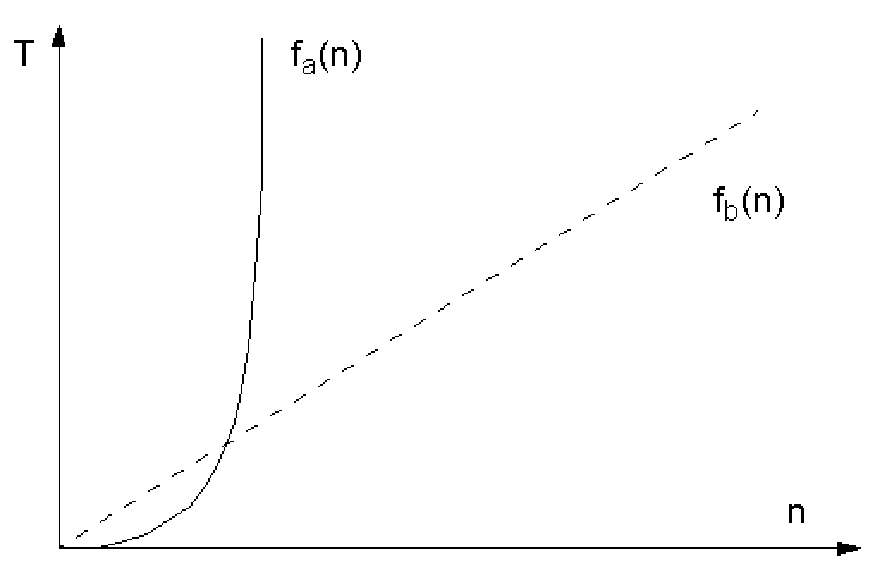
\includegraphics[width=0.9\textwidth]{function.png} 
\end{center}          
\end{frame}

\begin{frame}[fragile]{Interpretação da Complexidade de Tempo}
\lstset{language=C++,
          keywordstyle=\color{blue}\ttfamily,
          stringstyle=\color{red}\ttfamily,
          commentstyle=\color{OliveGreen}\ttfamily,
          breaklines=true,
          basicstyle=\ttfamily\footnotesize
          }
\begin{itemize}
\item Aspecto essencial que deve ser expresso pelo cálculo de complexidade:
\begin{itemize}
\item Qual é o comportamento assintótico predominante de um algoritmo em função do tamanho do conjunto de dados a ser processado.
\item Exemplo: se é linear, polinomial (quadrático, cúbico, etc.), logarítmico ou exponencial.
\end{itemize}
\end{itemize}
\end{frame}

\begin{frame}[fragile]{Análise Assintótica}
\lstset{language=C++,
          keywordstyle=\color{blue}\ttfamily,
          stringstyle=\color{red}\ttfamily,
          commentstyle=\color{OliveGreen}\ttfamily,
          breaklines=true,
          basicstyle=\ttfamily\footnotesize
          }
\begin{itemize}
\item Para a análise do comportamento de algoritmos existe toda uma terminologia própria;
\item Para o cálculo do comportamento de algoritmos foram desenvolvidas diferentes medidas de complexidade;
\item A mais importante delas e que é usada na prática é chamada de Ordem de Complexidade ou Notação-O ou Big-Oh.
\end{itemize}
\end{frame}

\begin{frame}[fragile]{Análise Assintótica}
\lstset{language=C++,
          keywordstyle=\color{blue}\ttfamily,
          stringstyle=\color{red}\ttfamily,
          commentstyle=\color{OliveGreen}\ttfamily,
          breaklines=true,
          basicstyle=\ttfamily\footnotesize
          }
\begin{itemize}
\item Definição (Big-Oh): $T(n) = O(f(n))$ se existem constantes $c$ e $n_0$ tais que $T(n)c.f(n)$ quando $n > n_{0}$;
\item A definição indica que existe uma constante c que faz com que $c.f(n)$ seja sempre pelo menos tão grande quanto $T(n)$, desde que n seja maior que um $n_0$;
\item Em outras palavras: a Notação-O me fornece a Ordem de Complexidade ou a Taxa de Crescimento de uma função;
\item Para isso, não consideramos os termos de ordem inferior da complexidade de um algoritmo, apenas o termo predominante.
\end{itemize}
\end{frame}

\begin{frame}[fragile]{Análise Assintótica}
\lstset{language=C++,
          keywordstyle=\color{blue}\ttfamily,
          stringstyle=\color{red}\ttfamily,
          commentstyle=\color{OliveGreen}\ttfamily,
          breaklines=true,
          basicstyle=\ttfamily\footnotesize
          }
\begin{itemize}
\item Exemplo: algoritmo com complexidade $T(n) = 3n^2 + 100n$.
\item Nesta função, o segundo termo tem um peso relativamente grande, mas a partir de $n_0 = 11$, é o termo $n^2$ que "dá o tom" do crescimento da função: uma parábola;
\item A constante 3 também tem uma influência irrelevante sobre a taxa de crescimento da função após um certo tempo;
\item Por isso dizemos que este algoritmo é da ordem de $n^2$ ou que tem complexidade $O(n^2)$.
\end{itemize}
\end{frame}

\begin{frame}[fragile]{Análise Assintótica}
\lstset{language=C++,
          keywordstyle=\color{blue}\ttfamily,
          stringstyle=\color{red}\ttfamily,
          commentstyle=\color{OliveGreen}\ttfamily,
          breaklines=true,
          basicstyle=\ttfamily\footnotesize
          }
\begin{itemize}
\item Exemplo: algoritmo com complexidade $T(n) = 3n^2 + 100n$.
\item Nesta função, o segundo termo tem um peso relativamente grande, mas a partir de $n_0 = 11$, é o termo $n^2$ que "dá o tom" do crescimento da função: uma parábola;
\item A constante 3 também tem uma influência irrelevante sobre a taxa de crescimento da função após um certo tempo;
\item Por isso dizemos que este algoritmo é da ordem de $n^2$ ou que tem complexidade $O(n^2)$.
\end{itemize}
\end{frame}

\begin{frame}[fragile]{Análise Assintótica}
\lstset{language=C++,
          keywordstyle=\color{blue}\ttfamily,
          stringstyle=\color{red}\ttfamily,
          commentstyle=\color{OliveGreen}\ttfamily,
          breaklines=true,
          basicstyle=\ttfamily\footnotesize
          }
          
\begin{center}
\begin{tabular}{c c}
Função & Nome \\
$1$ & Constante \\ 
$log$  $n$ & Logarítmica \\
$log^2$ $n$ & Log-quadrática\\
$n$ & Linear \\
$n$ $log$ $n$ & N-Logarítmica \\
$n^2$ & Quadrática \\
$n^3$ & Cúbica \\
$2^n$ & Exponencial 
\end{tabular}           
\end{center}
\end{frame}

\begin{frame}[fragile]{Cálculo da Complexidade de Tempo}
\lstset{language=C++,
          keywordstyle=\color{blue}\ttfamily,
          stringstyle=\color{red}\ttfamily,
          commentstyle=\color{OliveGreen}\ttfamily,
          breaklines=true,
          basicstyle=\ttfamily\footnotesize
          }
\begin{lstlisting}
inteiro somaCubos(inteiro n)
  inteiro i, somaParcial;
   início
1   somaParcial <- 0;
2   para i de 1 até n faça
3    somaParcial <- somaParcial + i * i * i;
4   fim para
5   retorne somaParcial;
   fim
\end{lstlisting}
\end{frame}

\begin{frame}[fragile]{Análise Assintótica}
\lstset{language=C++,
          keywordstyle=\color{blue}\ttfamily,
          stringstyle=\color{red}\ttfamily,
          commentstyle=\color{OliveGreen}\ttfamily,
          breaklines=true,
          basicstyle=\ttfamily\footnotesize
          }
\begin{itemize}
\item As declarações não tomam tempo nenhum;
\item A linha 4 também não toma tempo nenhum;
\item As linhas 1 e 5 contam uma unidade de tempo cada;
\item A linha 3 conta 4 unidades de tempo (2 multiplicações, uma adição e uma atribuição) e é executada n vezes, contando com um total de 4n unidades de tempo;
\item A linha 2 possui custos implícitos de inicializar i, testar se é menor que n e incrementá-lo. Contamos 1 unidade para a inicialização, n + 1 para os testes e n para os incrementos, o que perfaz 2n + 2 unidades de tempo;
\item O total perfaz 6n + 4 unidades de tempo, o que indica que o algoritmo é O(n), da Ordem de Complexidade n, ou seja, linear.
\end{itemize}
\end{frame}

\begin{frame}[fragile]{Regras para o cálculo}
\lstset{language=C++,
          keywordstyle=\color{blue}\ttfamily,
          stringstyle=\color{red}\ttfamily,
          commentstyle=\color{OliveGreen}\ttfamily,
          breaklines=true,
          basicstyle=\ttfamily\footnotesize
          }
\begin{itemize}
\item Laços: o tempo de execução de um laço é, no máximo, a soma dos tempos de execução das instruções dentro do laço (incluindo todos os testes) multiplicado pelo número de iterações;
\item Laços aninhados: analise-os de dentro para fora. O tempo total de execução de uma instrução dentro de um grupo de laços aninhados é o tempo de execução da instrução multiplicado pelo produto dos tamanhos dos laços.
\end{itemize}
\begin{lstlisting}
para i de 1 até n faça
 para j de 1 até n faça
  k <- k + 1;
 fim para
fim para
\end{lstlisting}
Exemplo: $O(n^2)$
\end{frame}

\begin{frame}[fragile]{Regras para o cálculo}
\lstset{language=C++,
          keywordstyle=\color{blue}\ttfamily,
          stringstyle=\color{red}\ttfamily,
          commentstyle=\color{OliveGreen}\ttfamily,
          breaklines=true,
          basicstyle=\ttfamily\footnotesize
          }
\begin{itemize}
\item Instruções Consecutivas: estes simplesmente somam, sendo os termos de ordem menor da soma ignorados.
\end{itemize}
\begin{lstlisting}
para i de 1 até n faça
 a[i] <- 0;
fim para
para i de 1 até n faça
 para j de 1 até n faça
  a[i] <- a[j] + k + 1;
 fim para
fim para
\end{lstlisting}
Exemplo: $O(n) + O(n^2) = O(n^2)$
\end{frame}

\begin{frame}[fragile]{Regras para o cálculo}
\lstset{language=C++,
          keywordstyle=\color{blue}\ttfamily,
          stringstyle=\color{red}\ttfamily,
          commentstyle=\color{OliveGreen}\ttfamily,
          breaklines=true,
          basicstyle=\ttfamily\footnotesize
          }
\begin{itemize}
\item O tempo de execução de um comando Se / Então / Senão nunca é maior do que o tempo de execução do teste cond em si mais o tempo de execução da maior dentre as expressões expressão1 e expressão2;
\item Ou seja: se expressão1 é $O(n^3)$  e expressão2 é $O(n)$, então o teste é $O(n^3) + 1 = O(n^3)$.
\end{itemize}
\begin{lstlisting}
se cond então
 expresssão1
senão
 expressão2
fim se
\end{lstlisting}
\end{frame}

\begin{frame}[fragile]{Regras para o cálculo}
\lstset{language=C++,
          keywordstyle=\color{blue}\ttfamily,
          stringstyle=\color{red}\ttfamily,
          commentstyle=\color{OliveGreen}\ttfamily,
          breaklines=true,
          basicstyle=\ttfamily\footnotesize
          }
\begin{itemize}
\item Chamada a Funções: segue a mesma regra dos laços aninhados - analise tudo de dentro para fora; 
\item Ou seja: para calcular a complexidade de um programa com várias funções, calcula-se primeiro a complexidade de cada uma das funções e depois considera-se cada uma das funções como uma instrução com a complexidade de função.
\end{itemize}
\end{frame}

\begin{frame}[fragile]{Regras para o cálculo}
\lstset{language=C++,
          keywordstyle=\color{blue}\ttfamily,
          stringstyle=\color{red}\ttfamily,
          commentstyle=\color{OliveGreen}\ttfamily,
          breaklines=true,
          basicstyle=\ttfamily\footnotesize
          }
\begin{itemize}
\item Recursão: é a parte mais difícil da análise de complexidade. Na verdade existem dois casos:
\begin{itemize}
\item Muitos algoritmos recursivos mais simples podem ser "linearizados", substituindo-se a chamada recursiva por alguns laços aninhados ou por uma outra subrotina extra e eventualmente uma pilha para controlá-la. Nestes casos, o cálculo é simples e pode ser feito depois da "linearização";
\item Em muitos algoritmos recursivos, porém, isto não é possível. Nestes casos obtemos uma relação de recorrência que tem de ser resolvida e é uma tarefa matemática menos trivial.
\end{itemize}
\end{itemize}
\end{frame}

\begin{frame}[fragile]{Regras para o cálculo}
\lstset{language=C++,
          keywordstyle=\color{blue}\ttfamily,
          stringstyle=\color{red}\ttfamily,
          commentstyle=\color{OliveGreen}\ttfamily,
          breaklines=true,
          basicstyle=\ttfamily\footnotesize
          }
\begin{itemize}
\item Recursão: é a parte mais difícil da análise de complexidade. Na verdade existem dois casos:
\begin{itemize}
\item Muitos algoritmos recursivos mais simples podem ser "linearizados", substituindo-se a chamada recursiva por alguns laços aninhados ou por uma outra subrotina extra e eventualmente uma pilha para controlá-la. Nestes casos, o cálculo é simples e pode ser feito depois da "linearização";
\item Em muitos algoritmos recursivos, porém, isto não é possível. Nestes casos obtemos uma relação de recorrência que tem de ser resolvida e é uma tarefa matemática menos trivial.
\end{itemize}
\end{itemize}
\end{frame}

\begin{frame}[fragile]{Logaritmos e outros Tempos de Execução}
\lstset{language=C++,
          keywordstyle=\color{blue}\ttfamily,
          stringstyle=\color{red}\ttfamily,
          commentstyle=\color{OliveGreen}\ttfamily,
          breaklines=true,
          basicstyle=\ttfamily\footnotesize
          }
\begin{itemize}
\item O aspecto mais complexo na análise de complexidade centra-se em torno do logaritmo; 
\item Para analisar-se um algoritmo de complexidade logarítmica e chegar-se a um resultado correto sobre a sua ordem exata de complexidade é necessária uma certa experiência e algum "jeito" matemático;
\item Algumas regras de aproximação podem ser dadas, por exemplo, algoritmos seguindo a técnica Dividir-Para-Conquistar são muitas vezes n log n.
\end{itemize}
\end{frame}

\begin{frame}[fragile]{Logaritmos e outros Tempos de Execução}
\lstset{language=C++,
          keywordstyle=\color{blue}\ttfamily,
          stringstyle=\color{red}\ttfamily,
          commentstyle=\color{OliveGreen}\ttfamily,
          breaklines=true,
          basicstyle=\ttfamily\footnotesize
          }
\begin{itemize}
\item Quando um algoritmo, em uma passada de uma iteração toma o conjunto de dados e o divide em duas ou mais partes, sendo cada uma dessas partes processada separada e recursivamente, este algoritmo utiliza a técnica dividir-para-conquistar e será possivelmente n log n;
\item Um algoritmo é log n se ele toma um tempo constante O(1) para dividir o tamanho do problema, usualmente pela metade;
\item A pesquisa binária é um exemplo de log n.
\end{itemize}
\end{frame}

\begin{frame}[fragile]{Logaritmos e outros Tempos de Execução}
\lstset{language=C++,
          keywordstyle=\color{blue}\ttfamily,
          stringstyle=\color{red}\ttfamily,
          commentstyle=\color{OliveGreen}\ttfamily,
          breaklines=true,
          basicstyle=\ttfamily\footnotesize
          }
\begin{itemize}
\item Se o algoritmo toma tempo constante para reduzir o tamanho do problema em um tamanho constante, ele será O(n);
\item Se um algoritmo testa todas as combinações de alguma coisa, ele será exponencial;
\item Exemplo: Problema do Caixeiro Viajante
\end{itemize}
\end{frame}

\begin{frame}[fragile]{Checando a sua análise}
\lstset{language=C++,
          keywordstyle=\color{blue}\ttfamily,
          stringstyle=\color{red}\ttfamily,
          commentstyle=\color{OliveGreen}\ttfamily,
          breaklines=true,
          basicstyle=\ttfamily\footnotesize
          }
\begin{itemize}
\item Uma vez que a análise de complexidade tenha sido executada, é interessante verificar-se se a resposta está correta e é tão boa quanto possível;
\item Uma forma de se fazer isto é o procedimento pouco matemático de se codificar o trecho de algoritmo cuja complexidade se tentou descrever e verificar se o tempo de execução coincide com o tempo previsto pela análise;
\item Quando n dobra, o tempo de execução se eleva de um fator 2 para algoritmos lineares, fator 4 para quadráticos e fator 8 para cúbicos.
\end{itemize}
\end{frame}

\begin{frame}[fragile]{Checando a sua análise}
\lstset{language=C++,
          keywordstyle=\color{blue}\ttfamily,
          stringstyle=\color{red}\ttfamily,
          commentstyle=\color{OliveGreen}\ttfamily,
          breaklines=true,
          basicstyle=\ttfamily\footnotesize
          }
\begin{itemize}
\item Programas logarítmicos só aumentam o seu tempo de execução de uma constante a cada vez que n dobra. Algoritmos de O(n log n) tomam um pouco mais do que o dobro do tempo sob as mesmas circunstâncias;
\item Estes aumentos podem ser difíceis de se detectar se os termos de ordem inferior têm coeficientes relativamente grandes e n não é grande o suficiente;
\item Um exemplo é o pulo no tempo de execução de n=10 para n=100 em algumas implementações do problema da subseqüência de soma máxima.
\end{itemize}
\end{frame}

\begin{frame}[fragile]{Checando a sua análise}
\lstset{language=C++,
          keywordstyle=\color{blue}\ttfamily,
          stringstyle=\color{red}\ttfamily,
          commentstyle=\color{OliveGreen}\ttfamily,
          breaklines=true,
          basicstyle=\ttfamily\footnotesize
          }
\begin{itemize}
\item Distinguir programas n log n de programas lineares só em evidência de tempo de execução pode também ser muito difícil;
\item Uma boa praxe é, caso o programa não seja exponencial (o que você vai descobrir muito rápido), fazer alguns experimentos com conjuntos maiores de dados de entrada.
\end{itemize}
\end{frame}


\begin{frame}[fragile]{Trabalho Cálculo de Complexidade de Floyd}
\lstset{language=C++,
          keywordstyle=\color{blue}\ttfamily,
          stringstyle=\color{red}\ttfamily,
          commentstyle=\color{OliveGreen}\ttfamily,
          breaklines=true,
          basicstyle=\ttfamily\footnotesize
          }
\begin{itemize}
\item Considere o grafo e sua matriz de custos D, abaixo:
\end{itemize}
\begin{center}
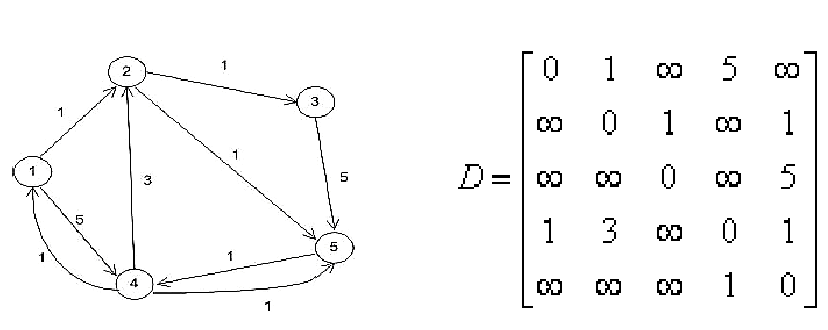
\includegraphics[width=0.9\textwidth]{floyd1.png} 
\end{center}   
\end{frame}

\begin{frame}[fragile]{Trabalho Cálculo de Complexidade de Floyd}
\lstset{language=C++,
          keywordstyle=\color{blue}\ttfamily,
          stringstyle=\color{red}\ttfamily,
          commentstyle=\color{OliveGreen}\ttfamily,
          breaklines=true,
          basicstyle=\ttfamily\footnotesize
          }
\begin{itemize}
\item Pelo algoritmo de Floyd pode-se obter a Matriz de Custos A e a Matriz de Roteamento R;
\item Exemplo: custo e rota v4 -> v3
\end{itemize}
\begin{center}
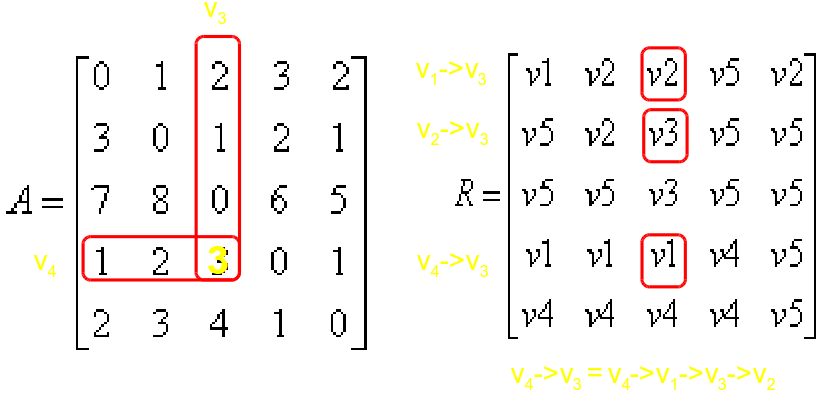
\includegraphics[width=0.9\textwidth]{floyd2.png} 
\end{center}   
\end{frame}

\begin{frame}[fragile]{Trabalho Cálculo de Complexidade de Floyd}
\lstset{language=C++,
          keywordstyle=\color{blue}\ttfamily,
          stringstyle=\color{red}\ttfamily,
          commentstyle=\color{OliveGreen}\ttfamily,
          breaklines=true,
          basicstyle=\ttfamily\footnotesize
          }
\begin{itemize}
\item Algoritmo de Floyd – modificado;
\item Considere a matriz de custos D[n,n] definida como no algoritmo de Floyd. O algoritmo produzirá uma matriz A[n,n], com comprimentos dos menores caminhos e ainda uma matriz R[n,n] que fornece o vértice k, que é o primeiro vértice a ser visitado no menor caminho de vi até vj;
\item \textbf{Entregue um documento PDF com todos os cálculos, com a função de tem T(n) e com a complexidade assintótica de O do algoritmo;}
\item A data esta definidida no moodle.
\end{itemize}
\end{frame}

\begin{frame}[fragile]{Trabalho Cálculo de Complexidade de Floyd}
\lstset{language=C++,
          keywordstyle=\color{blue}\ttfamily,
          stringstyle=\color{red}\ttfamily,
          commentstyle=\color{OliveGreen}\ttfamily,
          breaklines=true,
          basicstyle=\ttfamily\scriptsize
          }
\begin{lstlisting}
FloydModificado()
início
 para i = 1 até n faça
  para j = 1 até n faça
   A[i,j] <- D[i,j];
   R[i,j] <- 0;
  fim para
 fim para
 para i = 1 até n faça
  A[i,i] <- 0;
 fim para
 para k = 1 até n faça
  para i = 1 até n faça
   para j = 1 até n faça
    se A[i,k] + A[k,j] < A[i,j] então
     A[i,j] <- A[i,k] + A[k,j];
     R[i,j] <- k;
   fim para
  fim para
 fim para
fim
\end{lstlisting}
\end{frame}


{
\usebackgroundtemplate{
\includegraphics[width=\paperwidth,
height=\paperheight]{../reusable_images/fundo_capa.png}}
\begin{frame}

{\LARGE Perguntas????}

\end{frame}
}


{
\usebackgroundtemplate{
\includegraphics[width=\paperwidth,
height=\paperheight]{../reusable_images/fundo_capa.png}}
\begin{frame}

\includegraphics[scale=0.8]{../reusable_images/cc_logo_arge.png}\hspace{0.5cm}

\includegraphics[scale=0.95]{../reusable_images/by.png}

\vspace{1cm}
Este trabalho está licenciado sob uma Licença Creative Commons Atribuição 4.0 Internacional. Para ver uma cópia desta licença, visite http://creativecommons.org/licenses/by/4.0/.

\end{frame}
}
\end{document}
